\section{Auswertung}
\label{sec:Auswertung}

Für die Auswertung wird die Python-Bibliothek \texttt{numpy} benutzt. Die Fits entstehen mit \texttt{curve\_fit} aus \texttt{scipy.optimize}.
Die Fehlerrechnung wird mit \texttt{uncertainties} durchgeführt. Plots entstehen mit \texttt{matplotlib.pyplot}. \\

\subsection{Europium-152}

Die Messung von Europium ergibt folgendes Spektrum.

\begin{figure}[H]
    \centering
    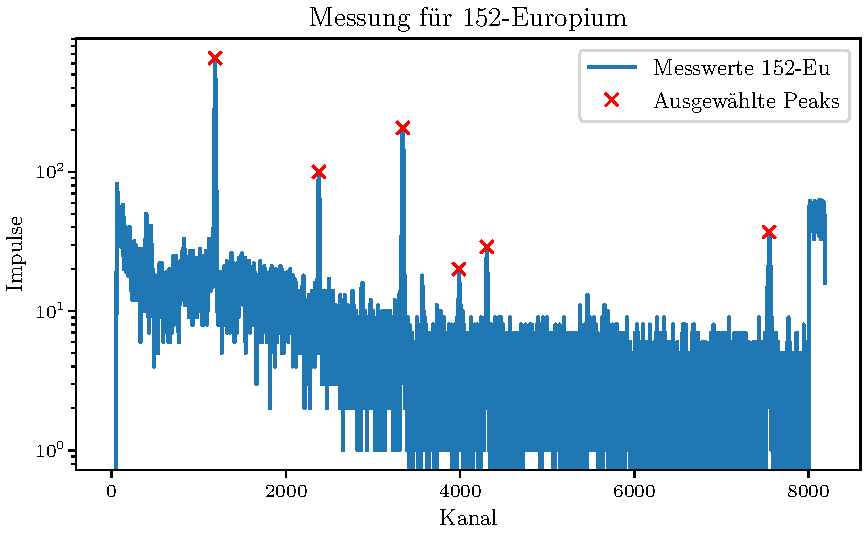
\includegraphics[width=\textwidth]{plots/Europium.pdf}
    \caption{Die Messung für Europium mit ausgewählten, markierten Peaks.}
    \label{fig:Europium}
\end{figure}

Die Kanäle können anhand ihrer relativen Lage und ihrer Impulsmenge bestimmten bekannten Energien zugeordnet werden.
%%%%%% CITE LNHB

\begin{table}[H]
    \centering
    \caption{Europium-Peaks.}
    \label{tab:europiumpeaks}
    \begin{tabular}{c c c c}
        \toprule
        {Energie ($\si{\kilo\electronvolt}$)} & {Wahrscheinlichkeit} & {Kanalnr.} & {Linieninhalt} \\
        \midrule
        121,78 &  28,6 & 1188 & 10375 \pm \, 101\\
        244,70 &  7,6  & 2380 & 1905  \pm \, 43\\
        344,30 &  26,5 & 3344 & 4081  \pm \, 63\\
        411,12 &  2,2  & 3986 & 406   \pm \, 20\\
        443,96 &  3,1  & 4308 & 488   \pm \, 22\\
        778,90 &  12,9 & 7550 & 841   \pm \, 29\\
        \bottomrule
    \end{tabular}
\end{table}

Das Verhältnis von Kanälen zu Energien kann linear beschrieben werden und gibt dann eine Funktion, mit der die Kanalnummer in eine Energie übersetzt werden kann.

\begin{figure}[H]
    \centering
    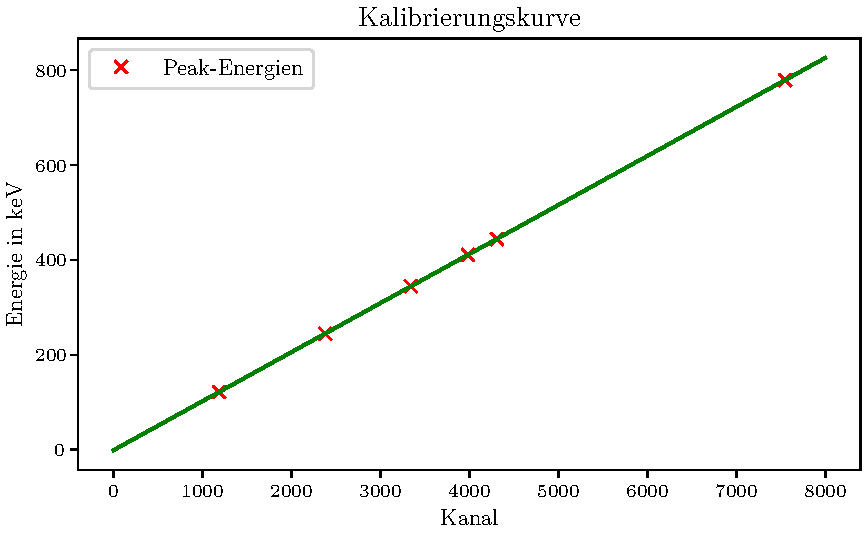
\includegraphics[width=\textwidth]{plots/EuKalibrierung.pdf}
    \caption{Energie und Kanalnummer, linear gefittet.}
    \label{fig:kalibrierung}
\end{figure}

Die Fitfunktion lautet
\begin{equation}
    E(K) = (0,103304 \pm 0,000044) \si{\kilo\electronvolt} \, \cdot K - (0,903881 \pm 0,188430) \, \si{\kilo\electronvolt}
    \label{eq:kanalenergie}
\end{equation}

Die Anfangsaktivität $A_0$ am 1. Oktober 2000 beträgt $A_0 = (4130 \pm 60) \, \si{\becquerel}$. Europium-152 hat eine Halbwertszeit von ungefähr $13,53$ Jahren.
Die Durchführung fand ungefähr $24,11$ Jahre später statt.
Die daraus errechnete Aktivität beträgt
\begin{equation}
    A = (1202 \pm 17) \, \si{\becquerel}.
    \label{eq:aktivitätEu}
\end{equation}

Der vorliegende Raumwinkel lässt sich geometrisch mit
\begin{equation}
    \Omega = 2 \pi (1 - \frac{a}{\sqrt{a^2 + r^2}}) = 0,20826 \pm 0,00023
\end{equation}
berechnen, wobei $a = (70,20 \pm 0,05) \, \si{\milli\meter} + \SI{15}{\milli\meter}$ der Abstand zwischen Probe und Hülle sowie Hülle und Detektor ist und $r = \SI{22,5}{\milli\meter}$ der Radius des Detektors ist.
 
Mit der Messdauer, $t = \SI{3553}{\minute}$, den Linieninhalten, den Wahrscheinlichkeiten und den Energien aus \ref{tab:europiumpeaks} können
die Effizienzen gemäß
\begin{equation}
    Q = \frac{4 \pi Z}{A W t \Omega}
    \label{eq:effizienz}
\end{equation}
berechnet werden, wobei $A$ die Aktivität, $W$ die Wahrscheinlichkeit zur Energie, $Z$ der Linieninhalt des Peaks ist.

\begin{table}[H]
    \centering
    \caption{Europium-Peaks.}
    \label{tab:europiumeffizienz}
    \begin{tabular}{c c}
        \toprule
        {Energie ($\si{\kilo\electronvolt}$)} & {Q} \\
        \midrule
        121,78 & $\num{5.126(90)e-5}$ \\
        244,70 & $\num{3.542(96)e-5}$ \\
        344,30 & $\num{2.176(46)e-5}$ \\
        411,12 & $\num{2.607(134)e-5}$ \\
        443,96 & $\num{2.224(105)e-5}$ \\
        778,90 & $\num{0.921(344)e-5}$ \\
        \bottomrule
    \end{tabular}
\end{table}

Die Effizienz in Abhängigkeit von der Energie kann als Potenzfunktion gefittet werden.

\begin{figure}[H]
    \centering
    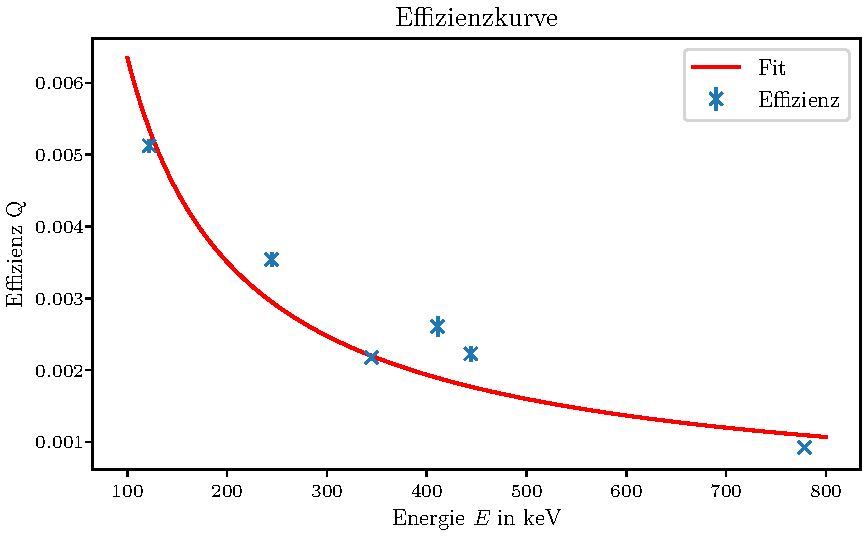
\includegraphics[width=\textwidth]{plots/EuEffizienz.pdf}
    \caption{Effizienz in Abhängigkeit der Energie.}
    \label{fig:effizienz}
\end{figure}

Der Fit ist gegeben durch
\begin{equation}
    Q(E) = \num{0.3290(307)} (\frac{E}{\si{\kilo\electronvolt}})^{\num{-0.8472(169)}}.
    \label{eq:fiteffizienz}
\end{equation}

\subsection{Cäsium-137}

Für Cäsium-137 wird folgendes Spektrum aufgenommen.

\begin{figure}[H]
    \centering
    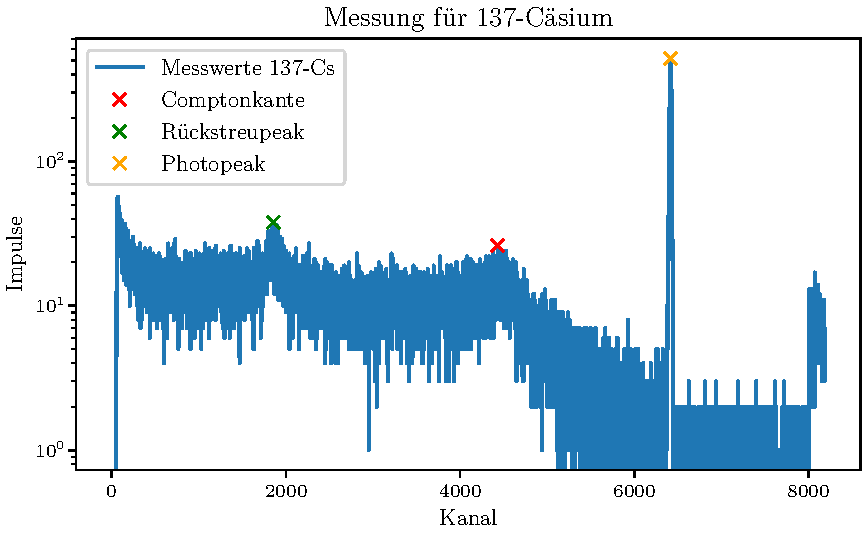
\includegraphics[width=\textwidth]{plots/Caesium.pdf}
    \caption{Die Messung für Cäsium mit ausgewählten, markierten Peaks.}
    \label{fig:Cäsium}
\end{figure}

Der Full Energy Peak befindet sich in Kanal $6415$, was einer Energie von $\qty{662(8)}{\kilo\electronvolt}$ entspricht.
Die Compton-Kante liegt bei einer Energie von $\qty{457(7)}{\kilo\electronvolt}$, der Rückstreupeak bei einer Energie von $\qty{191(4)}{\kilo\electronvolt}$.
Mit \eqref{eq:estrich} lassen sich diese Werte theoretisch überprüfen. Für den Compton-Peak findet sich eine Energie von $\qty{662(8)}{\kilo\electronvolt}$, für den Rückstreupeak ist keine genaue Energie berechenbar. \\

Ein Fit des differentiellen Wirkungsquerschnitts \eqref{eq:querschnitt} konnte nicht gemacht werden. Entsprechend ist eine sinnvolle Zählung des Inhalts des Comptonkontinuums auch nicht möglich. \\

Für den Photopeak des Cäsium-Spektrum lassen sich für einen Gauß-Fit der Form
\begin{equation}
    f(x) = \frac{a}{\sqrt{2\pi \sigma^2}} \cdot \exp^{-\frac{(x-\mu)^2}{2\sigma^2}}
    \label{eq:gauß}
\end{equation}

folgende Parameter bestimmen.

\begin{align}
    a &= \num{12233.183(110637)} \\
    \mu &= \num{6415.685(89)} \\
    \sigma &= \num{9.764(63)}
\end{align}

\begin{figure}[H]
    \centering
    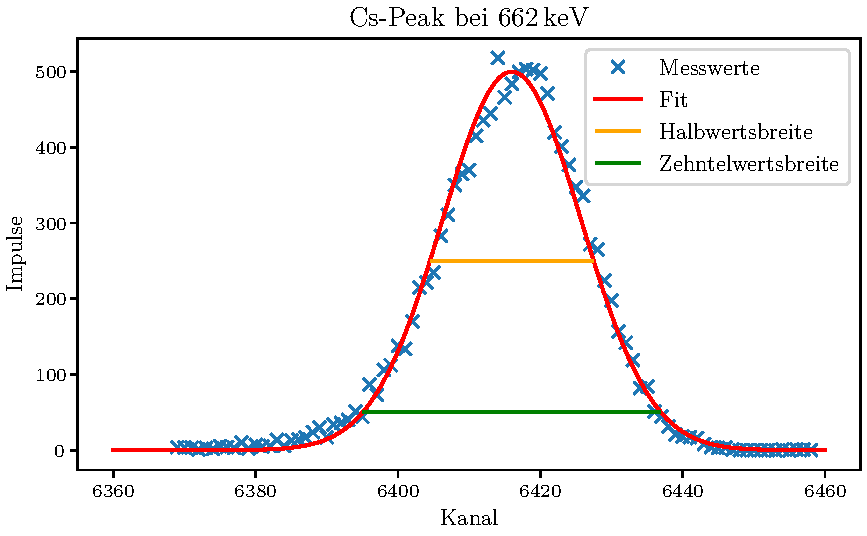
\includegraphics[width=\textwidth]{plots/CsPeak.pdf}
    \caption{Der Cäsium-Peak mit Fit, Halbwerts- und Zehntelwertsbreiten.}
    \label{fig:cspeak}
\end{figure}

Für die Halbwerts- und Zehntelwertsbreiten findt sich
\begin{table}[H]
    \centering
    \caption{Halbwerts- und Zehntelwertsbreiten}
    \label{tab:breiten}
    \begin{tabular}{c c c c}
        \toprule
        {Breite} & {Impulse} & {Breite (Kanäle)} & {Breite ($\si{\kilo\electronvolt}$)} \\
        \midrule
        Halbwertsbreite & 249,89 & 22,922 & $\qty{1.464(188)}{\kilo\electronvolt}$ \\
        Zehntelwertsbreite & 49,978 & 41,841 & $\qty{3.419(188)}{\kilo\electronvolt}$ \\
        \bottomrule
    \end{tabular}
\end{table}

Das Verhältnis von Zehntel- zu Halbwertsbreite $\frac{E_\text{Zehntel}}{E_\text{Halb}}$  einer Normalverteilkung ist konstant und kann zur Überprüfung genutzt werden. Es gilt
\begin{align}
        \frac{E_\text{Zehntel}}{E_\text{Halb}} &\approx  1,823 \\
        \frac{41,841}{22,922} &\approx 1,825
\end{align}

Die Absorptionswahrscheinlichkeiten lassen sich mit Hilfe der Extinktionskoeffizienten % HIER REF ZU BILD
und \eqref{eq:Absorptionswahrscheinlichkeit} berechnen.
\begin{align}
    \mu_\text{Photo} &= 0,007 \\
    P_\text{Photo} &= 2,693 \% \\
    \mu_\text{Compton} &= 0,37 \\
    P_\text{Compton} &= 76,37 \%
\end{align}


\subsection{Barium-133}

Für Barium lässt sich folgendes Spektrum aufzeichnen.

\begin{figure}[H]
    \centering
    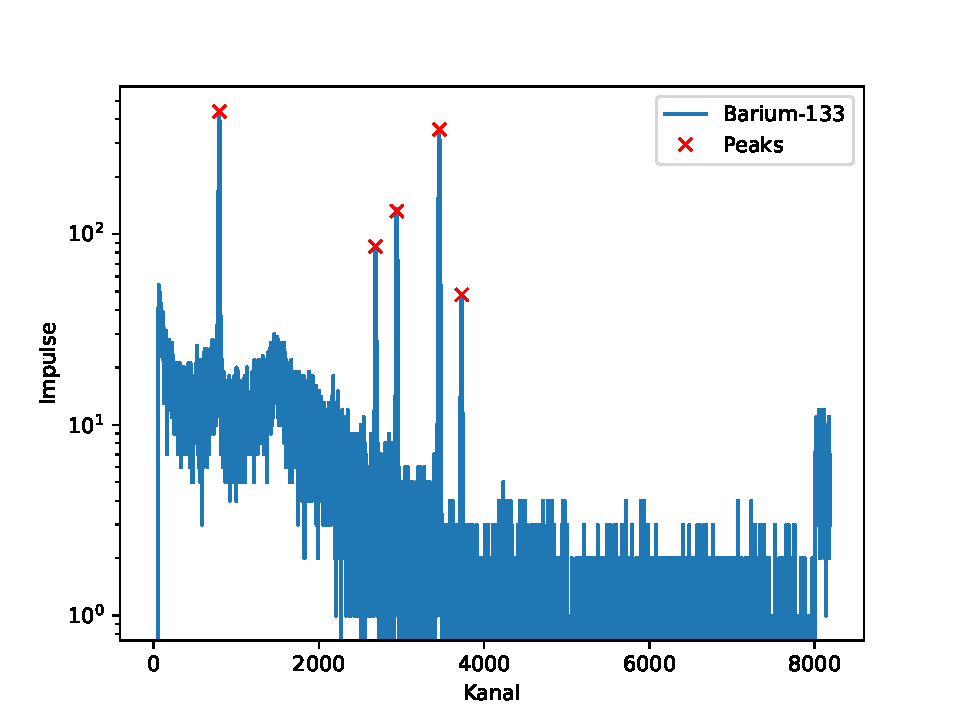
\includegraphics[width=\textwidth]{plots/Barium.pdf}
    \caption{Die Messung von Barium-133 mit ausgewählten, markierten Peaks.}
    \label{fig:barium}
\end{figure}

Die Kanäle, entsprechenden Energien, Wahrscheinlichkeiten und Effizienzen können \ref{fig:barium} entnommen werden.

\begin{table}[H]
    \centering
    \caption{Kanäle, Energien, Linieninhalte, Wahrscheinlichkeiten und Effizienzen von Barium-133.}
    \label{tab:barium}
    \begin{tabular}{c c c c c}
        \toprule
        {Kanalnr.} & {Energie ($\si{\kilo\electronvolt})$} & {Inhalt} & {Wahrscheinlichkeit (\%)} & {Effizienz ($\num{1e-3}$)} \\
        \midrule
        793  & \num{81.02(19)}  & \num{6879(33)} & \num{33.31(3)}  & \num{7.60(1)} \\
        2684 & \num{276.37(22)} & \num{1095(33)} & \num{7.13(6)}   & \num{2.65(1)} \\
        2944 & \num{303.23(23)} & \num{2258(47)} & \num{18.31(11)} & \num{2.45(1)} \\
        3456 & \num{356.12(24)} & \num{6183(78)} & \num{62.05(19)} & \num{2.13(1)} \\
        3727 & \num{384.11(25)} & \num{855(29)}  & \num{8.94(6)}   & \num{2.00(1)} \\
        \bottomrule
    \end{tabular}
\end{table}

Die Effizienzen werden dabei mit \eqref{eq:fiteffizienz} berechnet. Mit \eqref{eq:effizienz} 
können Aktivitäten berechnet werden, wobei die Messzeit hier $\qty{3461}{\second}$ lautet. Die mittlere Aktivität ermittelt sich zu
\begin{equation}
    \bar{A}_\text{Ba} = \num{801(10)}
\end{equation}

\subsection{Unbekanntes Erz}

Für das unbekannte Erz wird folgendes Spektrum aufgenommen.

\begin{figure}[H]
    \centering
    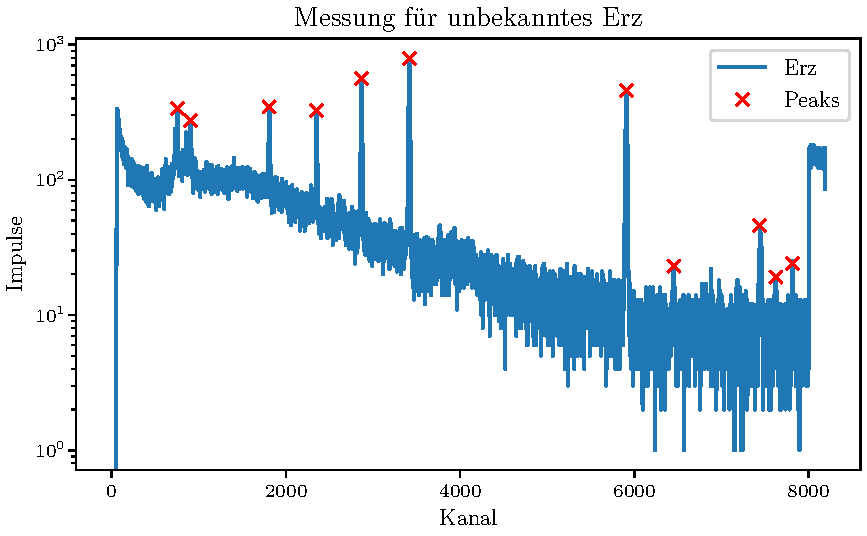
\includegraphics[width=\textwidth]{plots/H.pdf}
    \caption{Spektrum des unbekannten Erzes mit deutlich erkennbaren Peaks.}
    \label{fig:erz}
\end{figure}

\begin{table}[H]
    \centering
    \caption{Kanäle, Energien, Elemente, Linieninhalte, Wahrscheinlichkeiten und Effizienzen vom Erz. \cite{Altprotokoll}}
    \label{tab:erz}
    \begin{tabular}{c c c c c c}
        \toprule
        {Kanalnr.} & {Energie ($\si{\kilo\electronvolt})$} & Element & {Inhalt} & {Wahrscheinlichkeit (\%)} & {Effizienz ($\num{1e-3}$)} \\
        \midrule
        755  & \num{77.09(19)}  & Th & \num{8215(90)}   & \num{3.75(8)}    & \num{7.934(16)} \\
        903  & \num{92.38(19)}  & Th & \num{6982(83)}   & \num{2.18(19)}   & \num{6.794(12)} \\
        1808 & \num{185.87(20)} & Ra & \num{7362(85)}   & \num{3.555(19)}  & \num{3.731(35)} \\
        2351 & \num{241.96(21)} & Pb & \num{6209(78)}   & \num{7.268(22)}  & \num{2.976(22)} \\
        2867 & \num{295.27(22)} & Pb & \num{9925(99)}   & \num{18.414(36)} & \num{2.509(16)} \\
        3417 & \num{352.08(24)} & Pb & \num{15003(122)} & \num{35.6(7)}    & \num{2.157(12)} \\
        5913 & \num{609.93(32)} & Bi & \num{10148(100)} & \num{45.49(19)}  & \num{1.347(60)} \\
        6455 & \num{665.92(34)} & Bi & \num{572(23)}    & \num{1.530(7)}   & \num{1.249(54)} \\
        7442 & \num{767.88(37)} & Bi & \num{1084(32)}   & \num{4.892(16)}  & \num{1.105(46)} \\
        7626 & \num{786.89(38)} & Pb & \num{459(21)}    & \num{1.064(13)}  & \num{1.082(45)} \\
        7818 & \num{806.73(39)} & Bi & \num{520(22)}    & \num{1.262(6)}   & \num{1.060(44)} \\
        \bottomrule
    \end{tabular}
\end{table}

Die berechneten Aktivitäten können folgender Tabelle entnommen werden.

\begin{table}[H]
    \centering
    \caption{Aktivität vom Erz.}
    \label{tab:erz_aktivität}
    \begin{tabular}{c c}
        \toprule
        {Kanalnr.} & {Aktivität ($\si{\becquerel}$)} \\
        \midrule 
        755 & \num{4650(112)} \\
        903 & \num{7940(698)} \\
        1808 & \num{9349(120)} \\
        2351 & \num{4835( 63)} \\
        2867 & \num{3618( 37)} \\
        3417 & \num{3289( 70)} \\
        5913 & \num{2789( 30)} \\
        6455 & \num{5040(212)} \\
        7442 & \num{3375(103)} \\
        7626 & \num{6710(323)} \\
        7818 & \num{6547(288)} \\
        \bottomrule
    \end{tabular}
\end{table}

Da sich die Werte für dieselben Isotope stark unterscheiden, wird auf eine Mittelwertbildung verzichtet.